%%%%%%%%%%%%%%%%%%%%%%%%%%%%%%%%%%%%%%%%%
% Beamer Presentation
% LaTeX Template
% Version 1.0 (10/11/12)
%
% This template has been downloaded from:
% http://www.LaTeXTemplates.com
%
% License:
% CC BY-NC-SA 3.0 (http://creativecommons.org/licenses/by-nc-sa/3.0/)
%
%%%%%%%%%%%%%%%%%%%%%%%%%%%%%%%%%%%%%%%%%

%----------------------------------------------------------------------------------------
%	PACKAGES AND THEMES
%----------------------------------------------------------------------------------------

\documentclass{beamer}

\newcommand{\EMSE}{ {\rm EMSE}}
\newcommand{\CC}{ {\rm CC}}
\newcommand{\MSE}{ {\rm MSE}}
\newcommand{\WIN}{\scriptscriptstyle {\rm WIE}}
\newcommand{\OROI}{\scriptscriptstyle {\rm out ROI}}
\newcommand{\Her}{\scriptscriptstyle H}
\newcommand{\T}{\scriptscriptstyle T}
\newcommand{\LMS}{\scriptscriptstyle {\rm LMS}}
\newcommand{\RDE}{\scriptscriptstyle {\rm RDE}}
\newcommand{\MRD}{\scriptscriptstyle {\rm MRD}}
\newcommand{\MSD}{\scriptscriptstyle {\rm MSD}}
\newcommand{\SBD}{\scriptscriptstyle {\rm SBD}}
\newcommand{\SDD}{\scriptscriptstyle {\rm SDD}}
\newcommand{\WIE}{\scriptscriptstyle {\rm WIE}}
\newcommand{\R}{\scriptscriptstyle {\rm R}}
\newcommand{\I}{\scriptscriptstyle {\rm I}}
\newcommand{\mT}{\scriptscriptstyle -T}
\newcommand{\vir}{,\hspace{-0.15ex}}
\newcommand{\M}{\scriptscriptstyle M}
\newcommand{\MMA}{\rm \scriptscriptstyle MMA}
\newcommand{\neigh}{\scriptscriptstyle {\rm neigh}}
\newcommand{\st}{\scriptscriptstyle {\rm st}}
\newcommand{\nd}{\scriptscriptstyle {\rm nd}}
\newcommand{\CSD}{\scriptscriptstyle {\rm CSD}}
\newcommand{\E}{{\rm E}}
\newcommand{\uM}{{\mathbf u}}
\newcommand{\rM}{{\mathbf r}}
\newcommand{\xM}{{\mathbf x}}
\newcommand{\yM}{{\mathbf y}}
\newcommand{\XM}{{\mathbf X}}
\newcommand{\w}{{\mathbf w}}
\newcommand{\wo}{{\mathbf{w}}_{\rm o}}
\newcommand{\q}{{\mathbf q}}
\newcommand{\qp}{{\mathbf {\dot{q}}}}
\newcommand{\Nuquad}{\|{\mathbf u(n)}\|^2}
\newcommand{\NuquadP}{\|{\mathbf u(n)}\|^2_{{\mathbf R}^{-1}(n)}}
\newcommand{\uMc}{{\mathbf u}^{\ast}}
\newcommand{\wtil}{\widetilde{\mathbf w}}
\newcommand{\Dw}{\boldsymbol{\Delta}{\mathbf w}}
\newcommand{\Dewp}{\boldsymbol{\Delta}{\mathbf{\dot{w}}}}
\newcommand{\Pb}{{\mathbf R}^{-1}}
\newcommand{\ebari}{{\bar{e}}_i}
\newcommand{\field}[1]{\mathbb{#1}}
\newcommand{\re}{\field{R}}
\newcommand{\co}{\field{C}}
\newcommand{\CO}{\field{C}}
\newcommand{\RE}{\field{R}}
\newcommand{\Tr}{{\rm Tr}}
\newcommand{\Ru}{{\mathbf R}}
\newcommand{\sgbeta}{\sigma_{\scriptscriptstyle{\!\alpha}}^2}
\newcommand{\sgphi}{\sigma_{\scriptscriptstyle{\!\varphi}}^2}
\newcommand{\cred}{\textcolor{red}}
\newcommand{\lbo}{\lambda_{\rm o}}
\newcommand{\cond}{\mathbf{w}_1(n\!-\!1),\mathbf{w}_{2}(n\!-\!1)}
\newcommand{\cb}{\textcolor{blue}}
\newcommand{\pu}{\mathbf{p}_{\!\scriptscriptstyle \Delta}}
\definecolor{laranja}{rgb}{0.8,0.5,0}
\newcommand{\crt}{\textcolor{laranja}}
\newcommand{\Psibf}{\boldsymbol{\Psi}}
\newcommand{\Sigmabf}{\boldsymbol{\Sigma}}
\newcommand{\epsbf}{\boldsymbol{\epsilon}}
\newcommand{\betabf}{\boldsymbol{\beta}}
\newcommand{\alphabf}{\boldsymbol{\alpha}}
\newcommand{\thetabf}{\boldsymbol{\theta}}
\newcommand{\gammabf}{\boldsymbol{\gamma}}
\newcommand{\lambdabf}{\boldsymbol{\lambda}}
\newcommand{\ML}{{\rm ML}}
\newcommand{\LS}{{\rm LS}}
\newcommand{\SSS}{{\rm SS}}
\newcommand{\UPS}{{\rm UPS}}
\newcommand{\PS}{{\rm PS}}

\mode<presentation> {

% The Beamer class comes with a number of default slide themes
% which change the colors and layouts of slides. Below this is a list
% of all the themes, uncomment each in turn to see what they look like.

%\usetheme{default}
%\usetheme{AnnArbor}
%\usetheme{Antibes}
%\usetheme{Bergen}
%\usetheme{Berkeley}
%\usetheme{Berlin}
%\usetheme{Boadilla}
\usetheme{CambridgeUS}
%\usetheme{Copenhagen}
%\usetheme{Darmstadt}
%\usetheme{Dresden}
%\usetheme{Frankfurt}
%\usetheme{Goettingen}
%\usetheme{Hannover}
%\usetheme{Ilmenau}
%\usetheme{JuanLesPins}
%\usetheme{Luebeck}
%\usetheme{Madrid}
%\usetheme{Malmoe}
%\usetheme{Marburg}
%\usetheme{Montpellier}
%\usetheme{PaloAlto}
%\usetheme{Pittsburgh}
%\usetheme{Rochester}
%\usetheme{Singapore}
%\usetheme{Szeged}
%\usetheme{Warsaw}

% As well as themes, the Beamer class has a number of color themes
% for any slide theme. Uncomment each of these in turn to see how it
% changes the colors of your current slide theme.

%\usecolortheme{albatross}
%\usecolortheme{beaver}
%\usecolortheme{beetle}
%\usecolortheme{crane}
%\usecolortheme{dolphin}
%\usecolortheme{dove}
%\usecolortheme{fly}
%\usecolortheme{lily}
%\usecolortheme{orchid}
%\usecolortheme{rose}
%\usecolortheme{seagull}
%\usecolortheme{seahorse}
%\usecolortheme{whale}
%\usecolortheme{wolverine}

%\setbeamertemplate{footline} % To remove the footer line in all slides uncomment this line
\setbeamertemplate{footline}[page number] % To replace the footer line in all slides with a simple slide count uncomment this line

\setbeamertemplate{navigation symbols}{} % To remove the navigation symbols from the bottom of all slides uncomment this line
}

\usepackage{graphicx} % Allows including images
\usepackage{booktabs} % Allows the use of \toprule, \midrule and \bottomrule in tables
\usepackage{color}
\usepackage{amsmath}
\usepackage{hyperref}

%----------------------------------------------------------------------------------------
%	TITLE PAGE
%----------------------------------------------------------------------------------------

\title[Optimization]{An Introduction to Optimization} % The short title appears at the bottom of every slide, the full title is only on the title page

\author{Jer\'onimo Arenas-Garc\'{\i}a, Jes\'us Cid Sueiro} % Your name
\institute[UC3M] % Your institution as it will appear on the bottom of every slide, may be shorthand to save space
{
Universidad Carlos III de Madrid \\ % Your institution for the title page
\medskip
\textit{jeronimo.arenas@uc3m.es} % Your email address
}
\date{September 12, 2018}
%\date{\today} % Date, can be changed to a custom date

\begin{document}

%######################################################
%######################################################
\begin{frame}
\titlepage % Print the title page as the first slide
\end{frame}

%######################################################
%######################################################
\begin{frame}

    \frametitle{Sources}

This presentation is based on the following online resources:

\small



    \begin{itemize}
  
    	\item \href{http://web.stanford.edu/~boyd/papers/pdf/cvx_opt_intro.pdf}{Convex Optimization Overview by Boid et al.}
    	\item \href{https://www.scipy-lectures.org/advanced/mathematical_optimization/}{Mathematical optimization with Scipy by Gael Varoquaux}
    	\item \href{https://www.analyticsvidhya.com/blog/2017/03/introduction-to-gradient-descent-algorithm-along-its-variants/}{An Introduction to Gradient Descent by Faizan Shaikh}
    
    \end{itemize}
    
You can follow the following notebooks to learn more about optimization methods implementations in Python:

\begin{itemize}

\item \href{https://github.com/hammadshaikhha/Math-of-Machine-Learning-Course-by-Siraj/tree/master/Gradient\%20Descent\%20for\%20Optimization}{Notebook on Gradient Descent for Optimization}
\item \href{https://github.com/dtnewman/gradient_descent}{Notebook on Stochastic Gradient Descent (very important when cost function is based on sum over data)}
\item\href{https://github.com/mmckerns/tutmom}{Tutorial Notebook providing an introduction to optimization with Scipy (intro.ipynb)}

\end{itemize}
    

\end{frame}

%######################################################
%######################################################
\begin{frame}

    \frametitle{Contents}


\Large



    \begin{enumerate}
  
    	\item Overview of Optimization Methods
    	\item Gradient and Hessian-Based Methods
    \end{enumerate}
    

\end{frame}


%######################################################
%######################################################
\section{1. Overview of Optimization}
\subsection{The role of optimization in Machine Learning}

%######################################################
%######################################################
\begin{frame}

	\frametitle{Mathematical optimization}
	
	Mathematical optimization consists in the minimization or maximization of an objective function, possibly subject to a set of constraints.
	
	\begin{block}{Definition}
	$\text{Minimize~~~~~}{\w}^\ast= \arg\min_\w f(\w)$\\
	$\text{Subject to~~~} f_i(\w) \leq 0, ~i=1,\cdots,m~~~~$ (inequality constraints)\\
	$\text{~~~~~~~~~~~~~~~~} g_i(\w) = 0, ~i=1,\cdots,p~~~~$ (equality constraints)
	
	\end{block}

	\begin{itemize}
		\item $\w \in \Re^d$ is a set of parameters, and $\w^\ast$ is the optimal solution 
		\item $f(\w)$ is the objective or goal function
		\item Solution may exist only if the {\bf feasible set} is not empty
		\item Box constraints can be considered as particular cases of inequality constraints
	\end{itemize}

\end{frame}

%######################################################
%######################################################
\begin{frame}

	\frametitle{Mathematical optimization in machine learning}
\begin{itemize}
\item In supervised Machine Learning we are typically given a set of data
$${\cal D} = \left\{{\xM^{(k)}, y^{(k)}}\right\}_{k=1}^K$$
where labels $y^{(k)}$ represent the desired output or prediction associated to data vector $\xM^{(k)}$.

\item The problem can be formulated as that of learning a function that models the relation between $\xM$ and $y$
$$y = h(\xM)$$

\item In parametric methods, the function is parameterized with a set of parameters, $h_\w(\xM)$, and learning the function is equivalent to learning a set of parameters $\w^\ast$, i.e.,
$$h^\ast (\xM) = h_{\w^\ast}(\xM)$$


%$$f$$

\end{itemize}

\end{frame}

%######################################################
%######################################################
\begin{frame}

	\frametitle{Mathematical optimization in machine learning (II)}
\begin{itemize}
\item A typical objective of machine learning methods is to pursue that the postulated model fits well the training data, what frequently results in cost functions similar to
$$f(\w) = \sum_{k=1}^K \ell(y^{(k)}, h_\w(\xM^{(k)}))$$
where $\ell(\cdot, \cdot)$ is an error function that measures discrepancy between the arguments. 

\item In this context, optimization methods can be used to minimize $f(\w)$, and therefore to obtain a good prediction model.

\item Different methods are characterized by different objective functions and possibly the presence of constraints.

\item Futhermore, regularization is sometimes considered to prevent solutions that fit extremely well the training data but generalize poorly to new data.

\end{itemize}

\end{frame}


%######################################################
%######################################################
\begin{frame}

	\frametitle{Mathematical optimization in machine learning (III)}
$$f(\w) = \sum_{k=1}^K \ell(y^{(k)}, h_\w(\xM^{(k)})) ~~~~~~ \color{red}{[+R(\w)]}$$
\begin{itemize}

\item Evaluation and optimization of the cost function can get challenging because of
	\begin{itemize}
	\item Availability of very large datasets (big data)
	\item The shape of $f(\w)$, with many local minima and maxima (e.g., in deep learning)
	\end{itemize}

\item In this sense, we can say that the renaissance of Machine Learning in the last 20-30 years has been possible, at least in part, thanks to the development of powerful and efficient optimization techniques, as well as the increasing availability of computing power.

\end{itemize}

\end{frame}

%######################################################
%######################################################
\subsection{Convex optimization}

%######################################################
%######################################################
\begin{frame}

	\frametitle{Convex optimization}

Most optimization problems are intractable. Convex optimization is a very important exception to this statement. 
	
	\begin{block}{Definition: Convex optimization problem}
	$\text{Minimize~~~~~}{\w}^\ast= \arg\min_\w f(\w)$\\
	$\text{Subject to~~~} f_i(\w) \leq 0, ~i=1,\cdots,m~~~~$ (inequality constraints)\\
	$\text{~~~~~~~~~~~~~~~~} {\bf A}{\w} = {\bf b}~~~~~~~~~~~~~~~~~~~~~~~~$ (equality constraints)
	
	\end{block}

	\begin{itemize}
		\item Equality constraints are linear
		\item Functions $f(\w)$ and $f_i(\w)$ are convex
	\end{itemize}

\end{frame}



%%######################################################
%%######################################################
%\begin{frame}
%
%	\frametitle{Why Convex optimization}
%
%	\begin{itemize}
%		\item beautiful, nearly complete theory
%		\begin{itemize}
%		\item (duality, optimality conditions, etc.)
%		\end{itemize}
%		\item Effective algorithms, methods (in theory and practice)
%		\begin{itemize}
%				\item get global solution (and optimality certificate)
%				\item polynomial complexity
%		\end{itemize}
%		\item Lots of applications (many more than previously thought)
%	\end{itemize}
%
%\end{frame}

%######################################################
%######################################################
\begin{frame}

	\frametitle{LP and QP optimization}

Linear Programming and Quadratic Programming are particular cases of convex optimization

	\begin{itemize}
		\item LP: Objective function and inequality constraints are also linear
		\item QP: Objective function is quadratic (in the parameters) and inequality constraints are linear
	\end{itemize}

Specific methods are available for both cases that are more efficient than using a generic solver for convex optimization


\end{frame}


%######################################################
%######################################################
\begin{frame}

	\frametitle{Convex optimization in practice}

Once you have successfully obtained a convex optimization formulation of your problem, you can usually solve it numerically

	\begin{itemize}
		\item Using available libraries for many programming languages.\\
		\begin{itemize}
			\item If problem is LP or QP, more efficient algorithms can be used.
			\item Reliably solved by interior-point methods on single machine
			\item Polynomial complexity
		\end{itemize}
		\item For Big Data problems, the previous implementations are not practical. You need to implement your own code.
		\begin{itemize}
			\item Gradient and Stochastic gradient methods
			\item Admit parallel implementations
			\item Frequently used in machine learning (e.g., deep learning)
		\end{itemize}
	\end{itemize}


\end{frame}


%######################################################
%######################################################
\section{2. Gradient and Hessian-Based Methods}
\subsection{Gradient Descent}
%######################################################
%######################################################
\begin{frame}

	\frametitle{Motivation of Gradient Descent}

\centerline{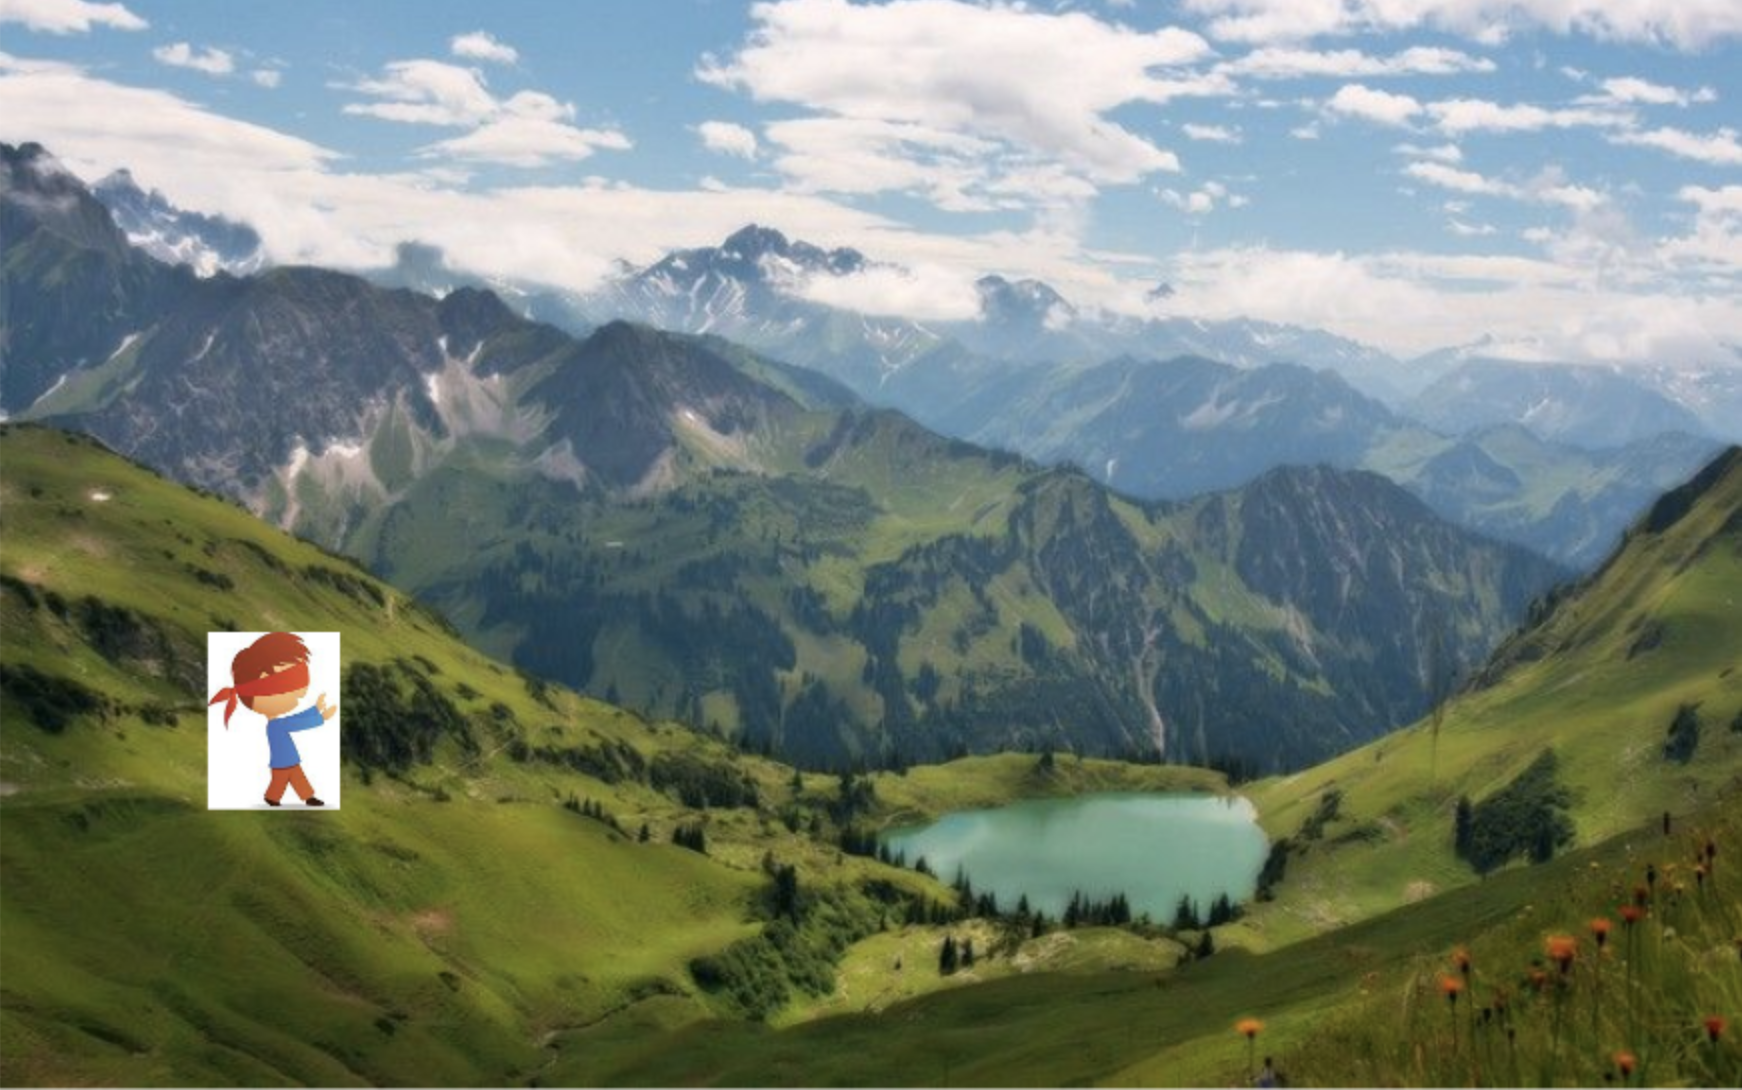
\includegraphics[width=11cm]{./figs/grad_desc1.png}}

Source: \url{http://cs231n.stanford.edu/slides/winter1516_lecture3.pdf}

\end{frame}

%######################################################
%######################################################
\begin{frame}

	\frametitle{Gradient Descent Algorithm}

\begin{itemize}
\item Very simple method for {\bf unconstrained} optimization
\item Iterate updates of the solution in the direction of maximum decrement of the function
$$\w_{n+1} = \w_n - \rho_n \nabla_\w f(\w)\mid_{\w=\w_n} $$
where $\rho_n>0$ is a learning step
\item Selection of the learning step is critical, since for small values we suffer small convergence, but too large values can result in algorithm divergence
\item Common choices are $\rho_n = \frac{1}{n}$ or $\rho_n = \frac{\alpha}{1 + \beta n}$
\item In general (non convex) problems only convergence to a local minimum is achieved
\item Can be initialized multiple times, keeping the best solution
\end{itemize}

\end{frame}


%######################################################
%######################################################
\begin{frame}

	\frametitle{Stochastic Gradient Descent (SGD) Algorithm}

\begin{itemize}
\item For very large training sets, repeated computation of $f(\w)$ and $\nabla_\w f(\w)$ gets prohibitive
$$\nabla_\w f(\w) = \sum_{k=1}^K \nabla_\w \ell(y^{(k)}, h_\w(\xM^{(k)})) ~~~~~~ \color{red}{[+\nabla_\w R(\w)]}$$

\item In Stochastic Gradient Descent the gradient is approximated by a sum over subsets of the training samples, i.e.,
$$\hat \nabla_\w f(\w) = \sum_{k \in {\cal D}_n} \nabla_\w \ell(y^{(k)}, h_\w(\xM^{(k)})) ~~~~~~ \color{red}{[+\nabla_\w R(\w)]}$$
where ${\cal D}_n \subset \left\{1,\dots,K \right\}$

\item The computational cost of each iteration of SGD is much smaller than that of gradient descent, though it usually needs more iterations to converge.
\end{itemize}


\end{frame}

%######################################################
%######################################################
\subsection{Newton's Method}

%######################################################
%######################################################
\begin{frame}

	\frametitle{Newton's Method Motivation}

	\begin{columns}
	
	\begin{column}{.3\textwidth}
		\vspace{.2cm}
		\centerline{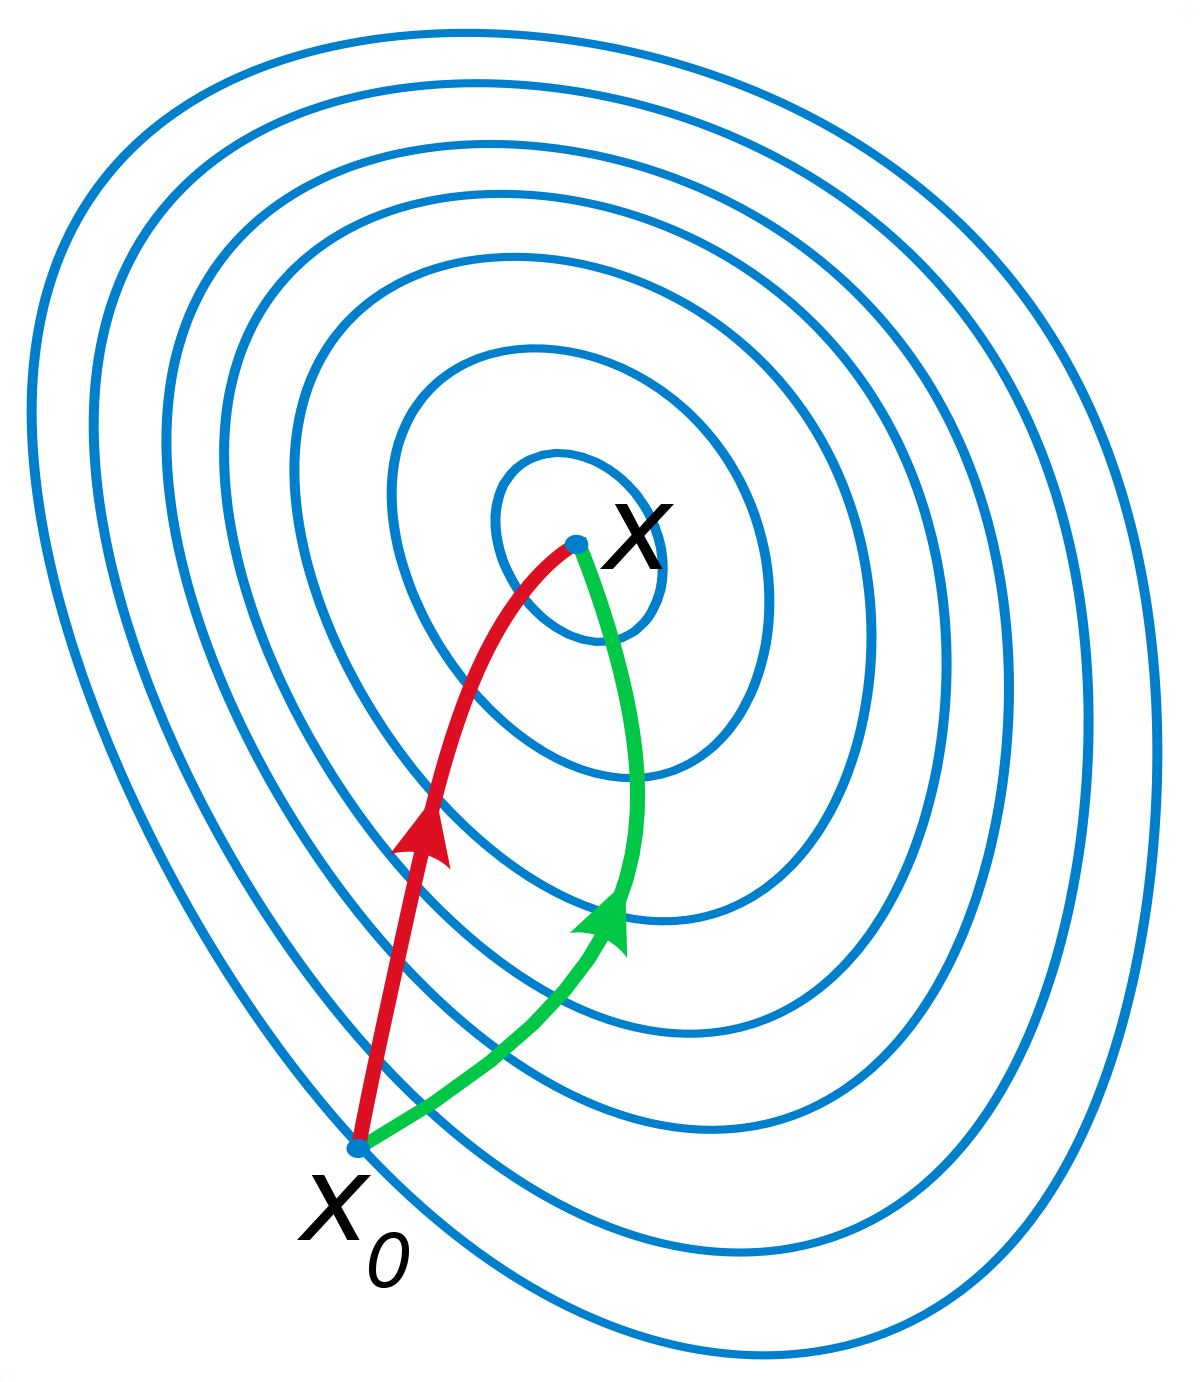
\includegraphics[width=3cm]{./figs/Newton_vs_Gradient.png}}
		
		Source: Wikipedia
	\end{column}
	
	\begin{column}{.7\textwidth}

		\begin{itemize}
		\item The direction of fastest decrement does not in general point towards the minimum of the objective function
		
		\item Gradient Descent in such case can result in slow convergence and oscillations during the convergence
		
		\item Better updates can be obtained by analyzing the local curvature of the error function, but this requires evaluation of second derivatives

		\end{itemize}

	\end{column}
	
	\end{columns}

\end{frame}


%######################################################
%######################################################
\begin{frame}

	\frametitle{Newton's Method}

		\begin{itemize}
		\item Approximation of $f(\w)$ by its second order Taylor series expansion around $\w_n$
		$$f(\w) = f(\w_n) + [\nabla_\w f(\w)\mid_{\w=\w_n}]^\top (\w - \w_n) + \frac{1}{2} (\w - \w_n)^\top {\bf H}(\w_n)(\w - \w_n)$$
		\item For the approximation, the minimum of $f(\w)$ is given by
		$$\w^\star = \w_n - [{\bf H}(\w_n)]^{-1} [\nabla_\w f(\w)\mid_{\w=\w_n}]$$
		\item Since the second order polynomial is just an approximation to $f(\w)$ we can expect $\w^\star$ to be just an approximation to the optimum solution
		\item We can then iterate the procedure, i.e.,
		$$\w_{n+1} = \w_n - \rho_n [{\bf H}(\w_n)]^{-1} [\nabla_\w f(\w)\mid_{\w=\w_n}]$$
		\item The cost per iteration is larger than for GD, but we can expect that less iterations are necessary

		\end{itemize}


\end{frame}


%######################################################
%######################################################
\begin{frame}

	\frametitle{Notebooks}

In this course, you will just need to implement Gradient Descent for Logistic Regression. Thus, you are advised to study, at least, the first of the following selected notebooks 

\begin{enumerate}

\item \href{https://github.com/hammadshaikhha/Math-of-Machine-Learning-Course-by-Siraj/tree/master/Gradient\%20Descent\%20for\%20Optimization}{Notebook on Gradient Descent for Optimization}
\item \href{https://github.com/dtnewman/gradient_descent}{Notebook on Stochastic Gradient Descent (very important when cost function is based on sum over data)}
\item\href{https://github.com/mmckerns/tutmom}{Tutorial Notebook providing an introduction to optimization with Scipy (intro.ipynb)}

\end{enumerate}

\end{frame}


\end{document} 